\documentclass{standalone}
\usepackage{chez}

\begin{document}
\chapter{October 02, 2020}

Recall that
\[
  H_q(S^n) = \begin{cases*}
    \ZZ & if \(q = 0, n\) \\[-1ex]
    0 & otherwise.
  \end{cases*}
\]
We claim that
\[
  H_q(S^\infty) = \begin{cases*}
    \ZZ & if \(q = 0\) \\[-1ex]
    0 & otherwise.
  \end{cases*}
\]

\begin{proposition}
  \(S^\infty\) is contractible.
\end{proposition}
\begin{proof}
  Since \(S^\infty = \bigunion S^n\),
  a point \(x \in S^\infty\) is a sequence
  \(x = (x_0, x_1, x_2, \dots)\) such that
  \begin{enumerate}[nosep]
    \item \(x_n = 0\) for all sufficiently large \(n\),
    \item \(\sum x_i^2 = 1\).
  \end{enumerate}
  Consider \(* \overset{f}\to S^\infty\)
  that picks out \((1, 0, 0, \dots)\).
  Also consider the map \(S^\infty \overset{g}\to *\)
  that maps every point in \(S^\infty\) to \(*\).

  We will show that \(f \circ g \simeq 1_{S^\infty}\)
  and \(g \circ g \simeq 1_{*}\).
  The second homotopy is easy because there
  is only one point that \(*\) can go to.
  To show the first, note that
  \(f \circ g \colon S^\infty \to S^\infty\)
  sends every point to \((1, 0, 0, \dots)\).

  Consider another map
  \begin{align*}
    T \colon& S^\infty \to S^\infty \\
      & (x_0, x_1, x_2, \dots) \mapsto (0, x_0, x_1, \dots).
  \end{align*}
  We will show that \(f \circ g \simeq T \simeq 1_{S^\infty}\).
  In particular, the homotopy \(T \simeq 1_{S^\infty}\) can be shown by
  \begin{align*}
    h \colon& S^\infty \times [0, 1] \to S^\infty \\
      & (x, t) \mapsto \frac{t x + (1-t) T x}{\norm{t x + (1-t) T x}}.
  \end{align*}
  This is well-defined and continues because \(t x + (1-t) T x\)
  is never the origin, since the first nonzero coordinate in \(T x\)
  occurs after the first nonzero coordinate in \(x\).

  We can show the homotopy \(T \simeq f \circ g\) with the homotopy
  \[
    h(x, t) = \frac{t T x + (1 - t)(1, 0, 0, \dots)}
                   {\norm{t T x + (1 - t)(1, 0, 0, \dots)}}.
  \]
  This is also well-defined because the first coordinate is always positive
  except for \(t = 1\), for which the value is \(T x\).
\end{proof}

This proof technique is called a swindle,
where in infinite dimensions we shift all the coordinates,
which works because there are an infinite number of dimensions.

\section{Real projective space}
For some \(k \in \NN\), \(\RP^k\) is \vocab{real projective \(k\)-space},
defined to be \(\RP^k \coloneq S^k / (x \sim -x)\).

\begin{example}
  \(\RP^0\) is \(S^0 / (x \sim -x)\), which is just \(*\).

  \(\RP^1\) is \(S^1 / (x \sim -x)\), which is another \(S^1\).

  \(\RP^2\) is \(S^2 / (x \sim x)\)
  is the sphere with antipodal points identified,
  but is hard to describe in more familiar terms.
  In fact, this is not embeddable in \(3\)-dimensional space.
\end{example}

Note that the inclusion of the equator \(S^k \to S^{k+1}\)
is compatible with \(x \mapsto -x\).
In particular, there are inclusions
\[
  \nullset \subseteq
  \RP^0 \subseteq
  \RP^1 \subseteq
  \RP^2 \subseteq \cdots
\]
In fact, this is a CW complex:
\[
  \begin{tikzcd}
    S^{k-1} \arrow[r] \arrow[d, hook] &
      \RP^{k-1} \arrow[d] \\
    D^k \arrow[r] &
      \RP^k
  \end{tikzcd}
\]
where \(S^{k-1} \to \RP^{k-1}\) is the quotient map,
\(S^{k-1} \to D^k\) is the boundary of \(D^k\),
where we think of \(D^k\) as the upper hemisphere of \(S^k\).

Then, we can define \(\RP^\infty = \bigunion \RP^n\), which is a finite type,
but not a finite CW complex.
Unlike \(S^\infty\), \(\RP^\infty\) is not contractible.


\section{Homology of CW complexes}
Before we start taking about homologies, let's introduce one more space.
\begin{definition}
  A \vocab{wedge of \(k\)-spheres} is a space, denoted by
  \(\bigvee_{i \in I} S^k\),
  consisting of \(\norm{I}\) different \(k\)-spheres all meeting
  at a single point.
\end{definition}

\begin{example}
  The figure eight is a wedge of two \(1\)-spheres,
  the wedge of three \(1\)-spheres is
  \begin{center}
    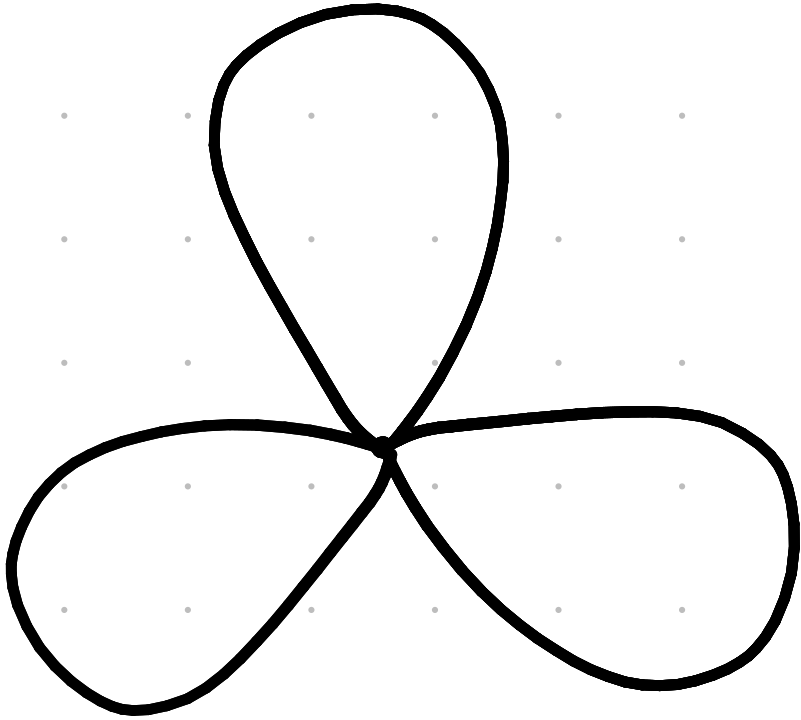
\includegraphics[width=0.15\textwidth]{18_905-201002-1.png}
  \end{center}
  and the wedge of two \(2\)-spheres is
  \begin{center}
    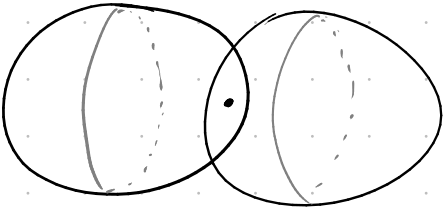
\includegraphics[width=0.25\textwidth]{18_905-200930-1.png}
  \end{center}
\end{example}
More formally, we can say
\(
  \bigvee_{i \in I} S^k =
  \left.\coprod_{i \in I} S^k \middle /
    \coprod_{i \in I} *\right.
\).

We can ask what are the reduced homology groups
\[
  \tilde H_q \parens[\Big]{\bigvee_{i \in I} S^k}
    = H_q \parens[\Big]{\bigvee_{i \in I} S^k, *}
    = H_q \parens[\Big]{\coprod_{i \in I} S^k, \coprod_{i \in I} *}.
\]
We consider the long exact sequence of the pair
\(\parens[\Big]{\coprod_{i \in I} S^k, \coprod_{i \in I} *}\).
\[
  \begin{tikzcd}
    \cdots \ar[r] &
    H_q \parens*{\coprod_{i \in I} *} \ar[r] &
    H_q \parens*{\coprod_{i \in I} S^k} \ar[r] &
    H_q \parens*{\coprod_{i \in I} S^k, \coprod_{i \in I} *}
      \ar[dll, "\delta"' pos=0.9, out=-20, in=160, looseness=0.7] & \\
  & H_{q-1} \parens*{\coprod_{i \in I} *} \ar[r] &
    H_{q-1} \parens*{\coprod_{i \in I} S^k} \ar[r] &
    H_{q-1} \parens*{\coprod_{i \in I} S^k, \coprod_{i \in I} *} \ar[r] &
    \cdots
  \end{tikzcd}
\]
Note that
\begin{align*}
  H_q \parens[\Big]{\coprod_{i \in I} S^k} &\iso \begin{cases*}
    \bigoplus_{i \in I} \ZZ & if \(q = 0, k\) \\[-1ex]
    0 & otherwise
  \end{cases*} \\
  H_q \parens[\Big]{\coprod_{i \in I} *} &\iso \begin{cases*} % chktex 1
    \bigoplus_{i \in I} \ZZ & if \(q = 0\) \\[-1ex] % chktex 1
    0 & if \(q \neq 0\).
  \end{cases*}
\end{align*}
with yields
\[
  \tilde H_q \parens[\Big]{\bigvee_{i \in I} S^k} \iso \begin{cases*}
    \bigoplus_{i \in I} \ZZ & if \(q = k\) \\[-1ex]
    0 & otherwise.
  \end{cases*}
\]

Now suppose \(X\) is a CW complex.
We want to find the relationship between
\(H_q(\Sk_{k-1} X)\) and \(H_q(\Sk_k X)\).

Consider the long exact sequence of the pair \((\Sk_k X, \Sk_{k-1} X)\):
\[
  \begin{tikzcd}
    \cdots \ar[r] &
    H_{q+1}(\Sk_k X, \Sk_{k-1} X) \ar[r] &
    H_q(\Sk_{k-1} X) \ar[r] &
    H_q(\Sk_k X) \ar[r] &
    H_q(\Sk_k X, \Sk_{k-1} X) \ar[r] &
    \cdots
  \end{tikzcd}
\]
Note that there is a pushout square
\[
  \begin{tikzcd}
    \coprod_{i \in I_k} S^{k-1} \arrow[r] \arrow[d] &
      \Sk_{k-1} X \arrow[d] \\
    \coprod_{i \in I_k} D^k \arrow[r] &
      \Sk_k X
  \end{tikzcd}
\]
This pushout diagram says that
\[
  \Sk_k X \big/ \Sk_{k-1} X
    \iso \coprod_{i \in I_k} D^k \Big/ \coprod_{i \in I_k} S^{k-1}
    \iso \bigvee_{i \in I_k} S^k,
\]
which means
\[
  H_q(\Sk_k X, \Sk_{k-1} X)
    = H_q(\Sk_k X / \Sk_{k-1} X, *)
    = \tilde H_q \parens[\Big]{\bigvee_{i \in I_k} S^k}
    = \begin{cases*}
      \bigoplus_{i \in I_k} \ZZ & if \(k = q\) \\[-1ex]
      0 & otherwise.
    \end{cases*}
\]






\end{document}
